% LaTeX Template for short student reports.
% Citations should be in bibtex format and go in references.bib
\documentclass[a4paper, 11pt]{article}
\usepackage[top=3cm, bottom=3cm, left = 2cm, right = 2cm]{geometry} 
\geometry{a4paper} 
\usepackage[utf8]{inputenc}
\usepackage{textcomp}
\usepackage{graphicx} 
\usepackage{amsmath,amssymb}  
\usepackage{bm}  
\usepackage[pdftex,bookmarks,colorlinks,breaklinks]{hyperref}  
\hypersetup{linkcolor=black,citecolor=black,filecolor=black,urlcolor=black} % black links, for printed output
\usepackage{memhfixc} 
\usepackage{pdfsync}  
\usepackage{fancyhdr}
\usepackage{fancyvrb}
\usepackage{natbib}
\usepackage{url}
%\pagestyle{fancy}
\usepackage{tabto}
\usepackage[shortlabels]{enumitem}
\usepackage{tikz}
\usepackage{verbatim}
\usepackage{nameref}
\usepackage{caption}
\usepackage{subcaption}
\usepackage{mathtools}

\title{Concrete Earth: A DirectX Game}
\author{Sam Drysdale}
\date{May 16, 2023}

\begin{document}
\graphicspath{{./Images/}}
\maketitle
\tableofcontents
\begin{flushleft}

\section{Summary}

\textit{Concrete Earth} is a game about nuclear semiotics. Ostensibly, the story is set in a medieval fiefdom, cursed by the occult ciphers long-etched into its landscape. The twist is this occurs millenia \textit{after} a nuclear apocalypse - the `curse' is radiation poisoning, the ciphers the dead language of the previous civilisation, warning of nearby waste repositories. Though it is still in development, this prototype demostrates how the DirectX 11 functionality might bring the concept to life. Indeed, for a game so concerned with language, it is appropriate that many key features are grounded in linguistics; while the terrain itself is generated by marching cubes, \textit{Concrete Earth} uses grammars to create both procedural screen shaders and a procedural narrative.



\newpage
\section{User Controls}

The user plays as a carriage driver, journeying forwards over an endless map. Periodically, they will be stopped by a `multiple-choice' event; an option must be selected before continuing. Such is the core game loop of \textit{Concrete Earth}.

\vspace{5pt}\noindent
The application uses the following key mappings:\footnote{While the framework registers inputs on press, note that options are only selected \textit{on release}.}

\begin{center}
\parbox[t]{0.75\textwidth}{
\vspace{0pt}\noindent 
\textbf{W} \dotfill{} Move north

\vspace{2.5pt}\noindent 
\textbf{A} \dotfill{} Move northwest

\vspace{2.5pt}\noindent 
\textbf{D} \dotfill{} Move northeast

\vspace{2.5pt}\noindent 
\textbf{1} \dotfill{} Select option \#$1$

\vspace{2.5pt}\noindent 
\textbf{2} \dotfill{} Select option \#$2$

\vspace{2.5pt}\noindent 
\textbf{3} \dotfill{} Select option \#$3$

\vspace{2.5pt}\noindent 
\textbf{Esc} \dotfill{} Quit
}\linebreak
\end{center}

Clicking \textbf{LMB} will also select an option. The application runs at a fixed $1920 \times 1080$ resolution.

\section{Features}\label{Features}

The following is a technical discussion of the key features of \textit{Concrete Earth}, with a focus on its advanced procedural generation. Mathematical models and code snippets are kept to a minimum, edited for clarity rather than accuracy to the original application.

%\subsection{Noise} % TECHNIQUE: Perlin/simplex noise...

\subsection{Procedural Terrain} % TECHNIQUE: Marching cubes...

Given the concept, this game's terrain is of course intended to evoke a sense of ``shunned land'' \citep{trth93}. In generating the jutting thorns and blocks so essential to the post-nuclear setting, though, there comes a problem - concavity. Height maps are perfectly adequate for creating rolling hills and valleys, but the fact that each of their $(x,z)$-coordinates can correspond to only one $y$-value would prevent any overhangs in \textit{Concrete Earth}'s barren landscape (see Figure \ref{Concave Terrain}).

%\vspace{5pt}\noindent
\begin{figure}[h]
\centering
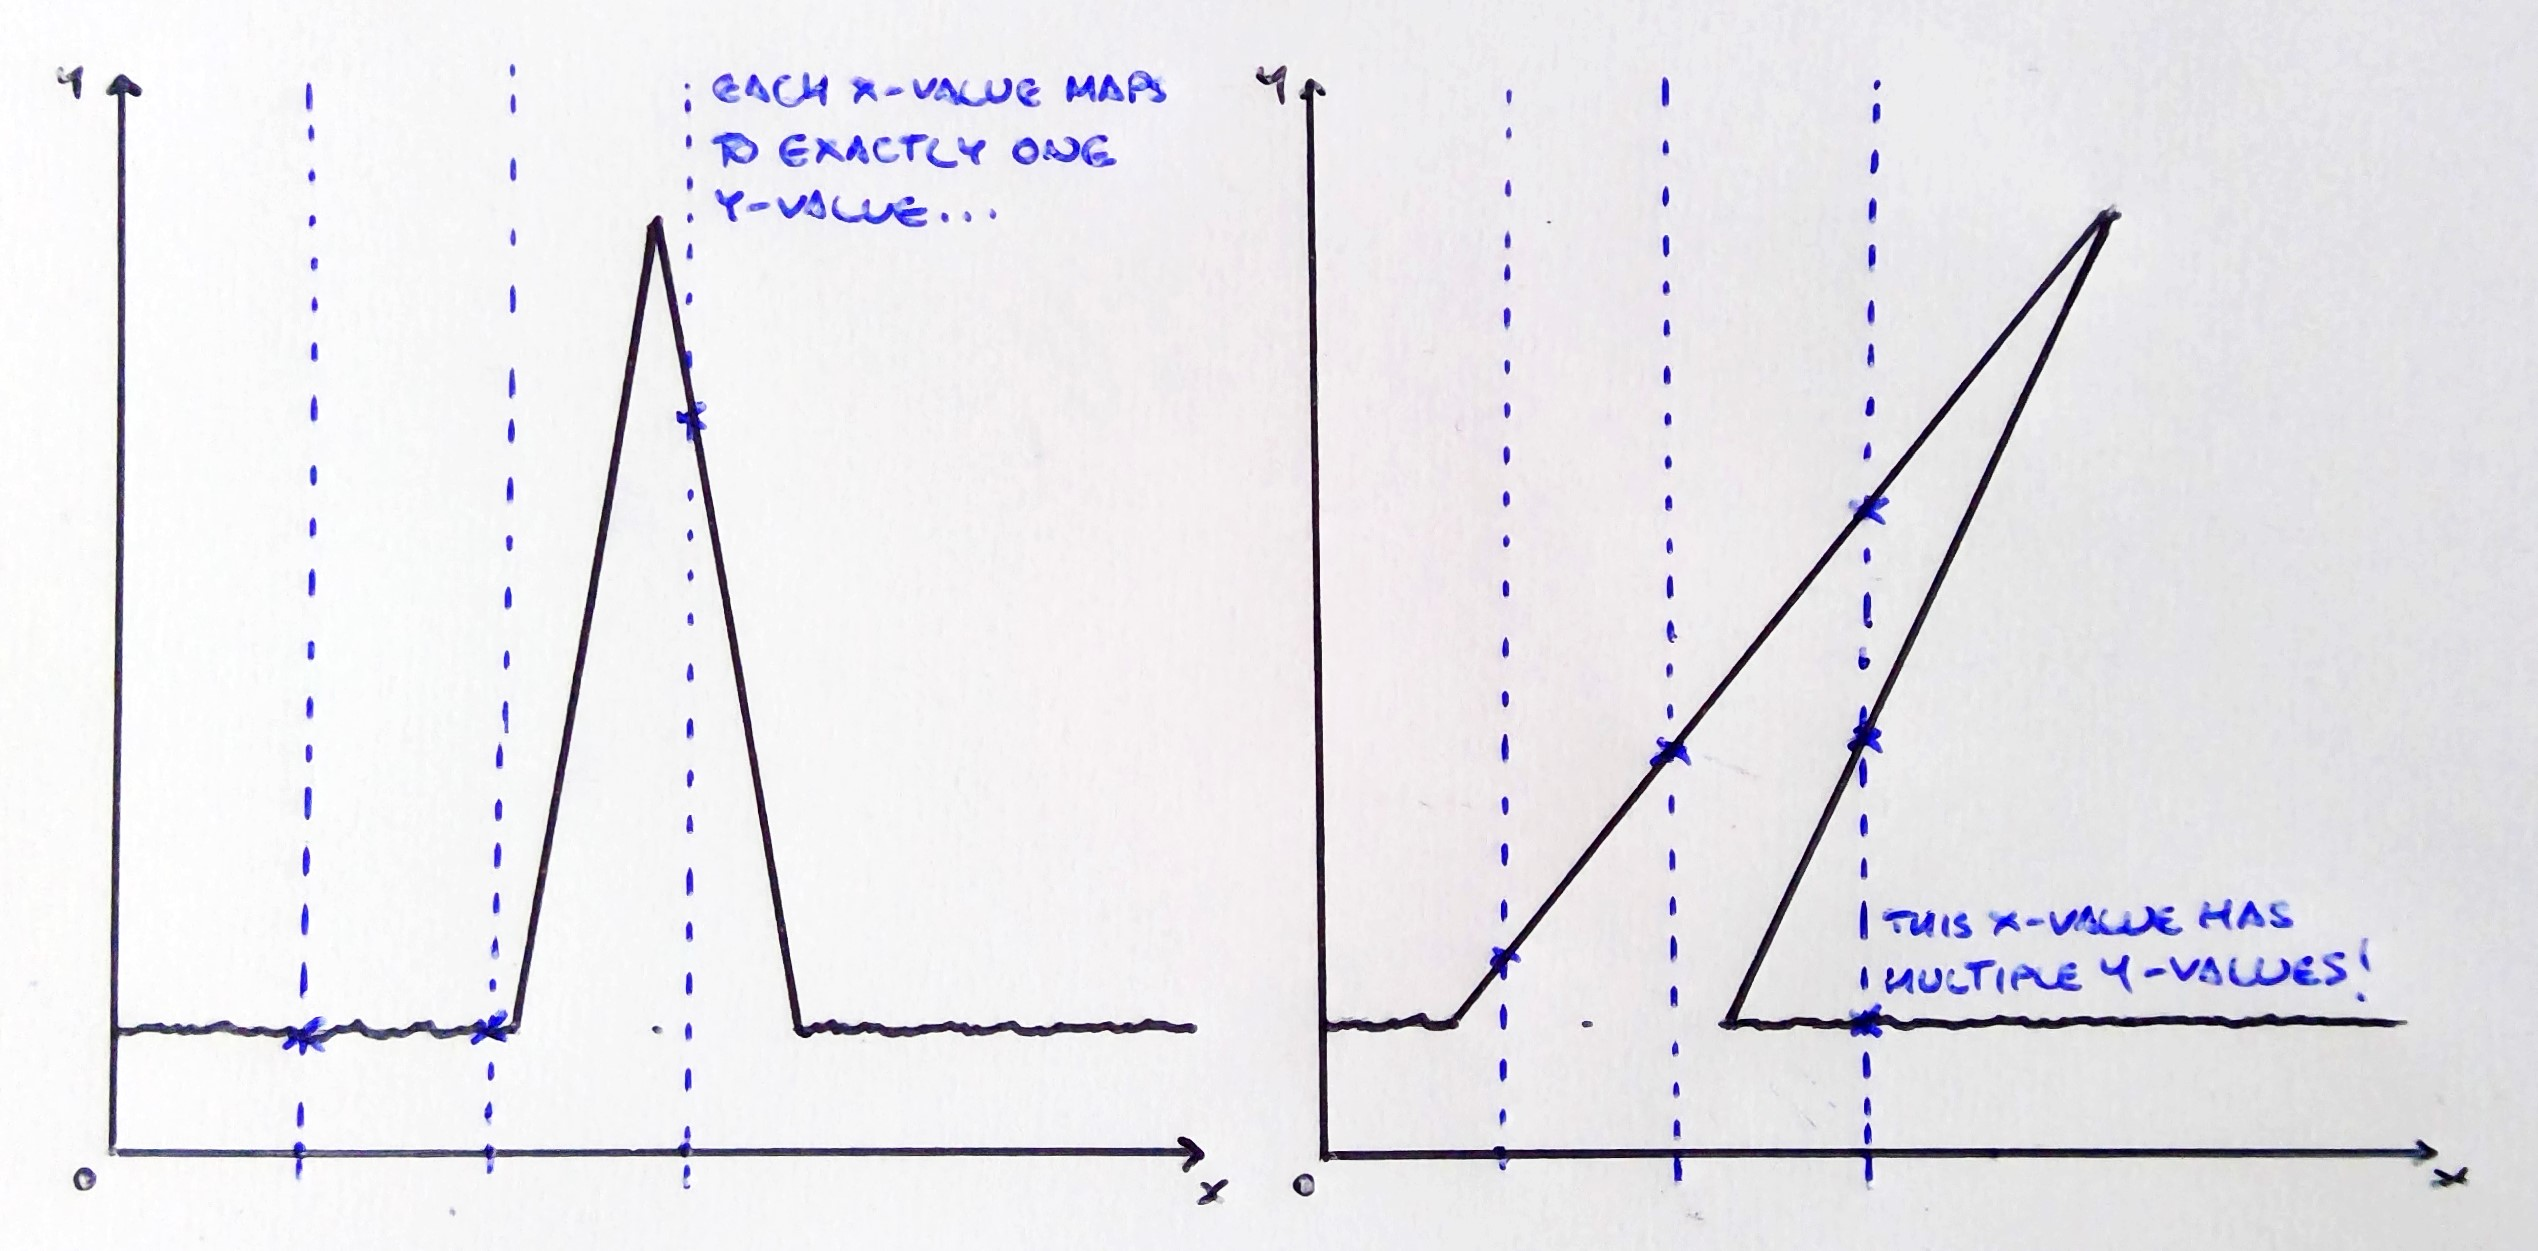
\includegraphics[width=0.66\textwidth]{Concave Terrain}
\caption{Two sketches of `thorny' terrain; the former can be generated by a height map, whereas the latter is too concave.}
\label{Concave Terrain}
\end{figure}

%\vspace{5pt}\noindent
%\newpage\noindent
Consider the two-dimensional analogue of this problem: how does one construct the bounding curve of a (potentially concave, or even disconnected) area? Taking an $(n+1) \times (n+1)$ grid, with $n \in \mathbb{N}$,\footnote{This could equally be an $(n+1) \times (m + 1)$ grid; keeping the dimensions the same is just `neater'.} let the scalar field $f : [0,1]^2 \rightarrow \mathbb{R}$ assign each gridpoint $(i,j)$ a corresponding value $f_{i,j} = f(i/n,j/n)$. Figure \ref{Marching Square Partitions} shows how to partition a cell so as to enclose the gridpoints with $f_{i,j} < c$ constant. Drawing such a partition into every cell of the grid will therefore approximate the \textit{isoline}\footnote{Informally, a `contour line' of the $2D$ field.} $f(x,y) = c$, with increasing accuracy as $n \rightarrow \infty$.%In each cell of the grid, straight lines can be drawn to  For each square cell, a line can be Consider%Under this construction, it is possible to approximate the \textit{isoclines}\footnote{Informally, the `contour lines' of the field.} $f(x,y) = c$ constant. Suppose%[By partitioning each of the $n \times n$ square cells according to which of its four gridpoints have $f_{i,j} < c$ (see Figure \ref{Marching Square Partitions}), an increasingly accurate curve emerges as $n \rightarrow \infty$.]

\vspace{5pt}\noindent
\begin{figure}[h]
\centering
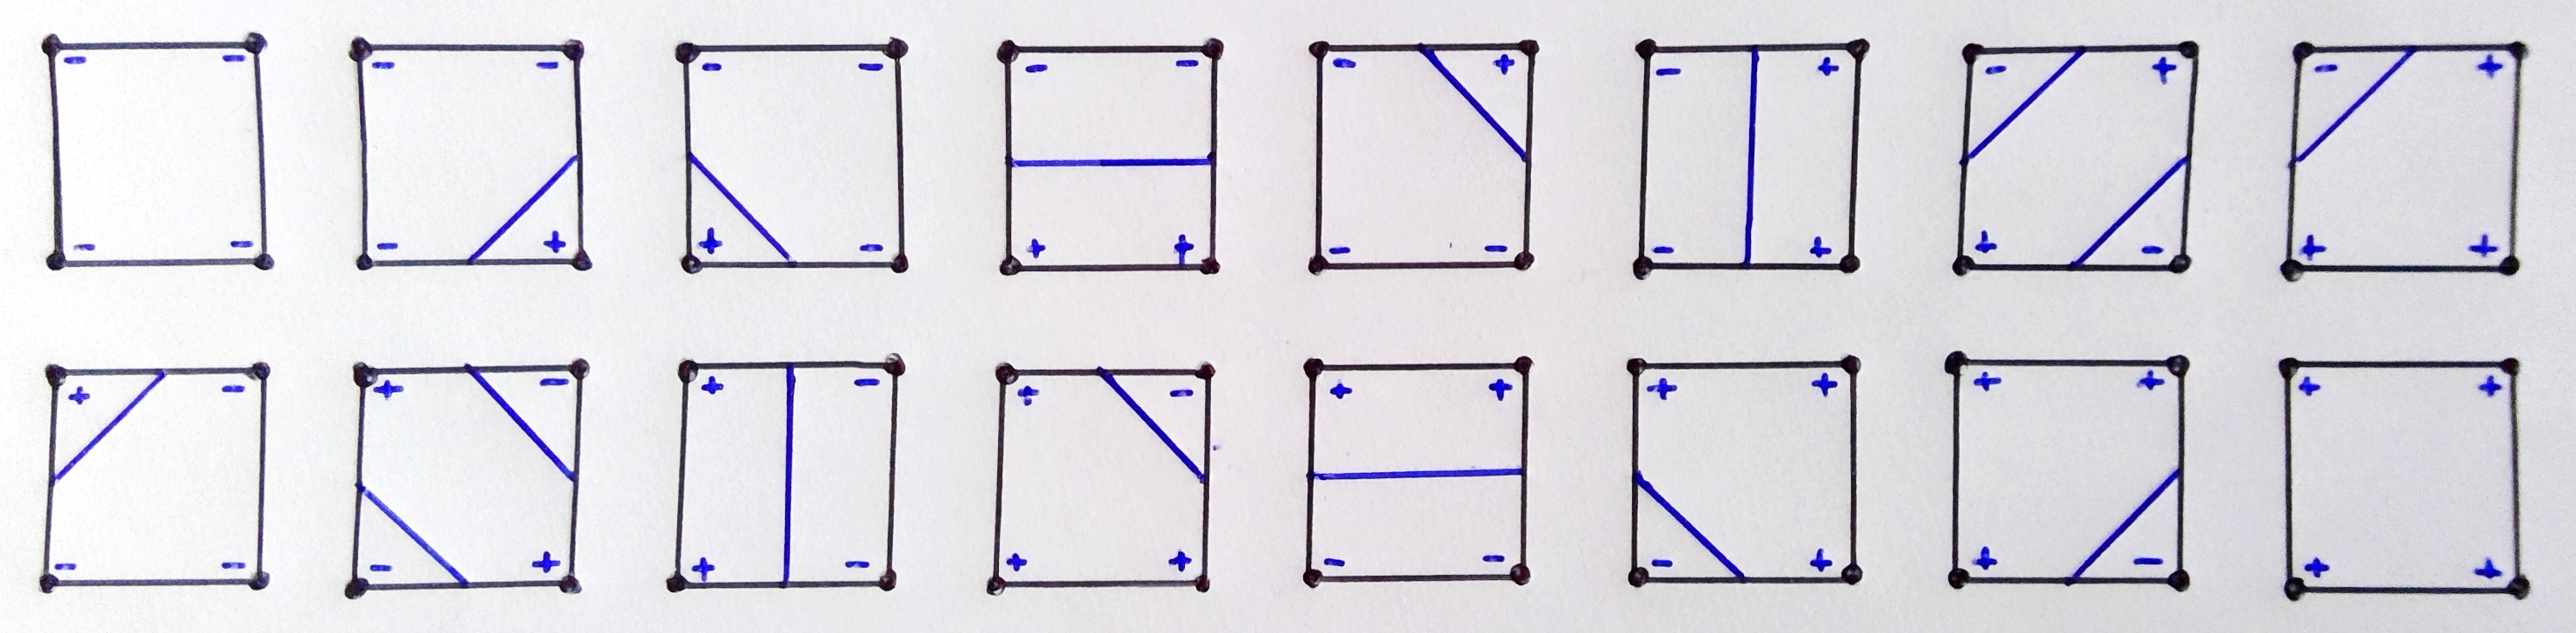
\includegraphics[width=0.9\textwidth]{Marching Square Partitions}
\caption{Partitions of a marching square. With each of the $4$ gridpoints existing in one of $2$ states (`$+$' for $f_{i,j} \geqslant c$, `$-$' for $f_{i,j} < c$), exactly $2^4 = 16$ partitions are possible.} % NB: $4$, ignoring symmetries!
\label{Marching Square Partitions}
\end{figure}

\vspace{5pt}\noindent
This is the \textit{marching squares} algorithm, so named for how it uses a \texttt{for} loop to `march through' and fill in each of the $n \times n$ square cells. Though a challenge to conceptualise, intuition can be built by running the 2D algorithm with pen and paper; Figure \ref{Marching Squares} contains manual constructions for %illustrates this analogue approach in relation to  Figure \ref{Marching Squares} shows a 2D  illustrates such an analogue approach as it relates to
$$f(x,y) = \min\left(\left(x-0.5\right)^2+\left(y-0.5\right)^2,4\left(\left(x-0.75\right)^2+\left(y-0.75\right)^2\right)\right),$$
a scalar field describing two overlapping circles.

\vspace{5pt}\noindent
\begin{figure}[h]
\centering
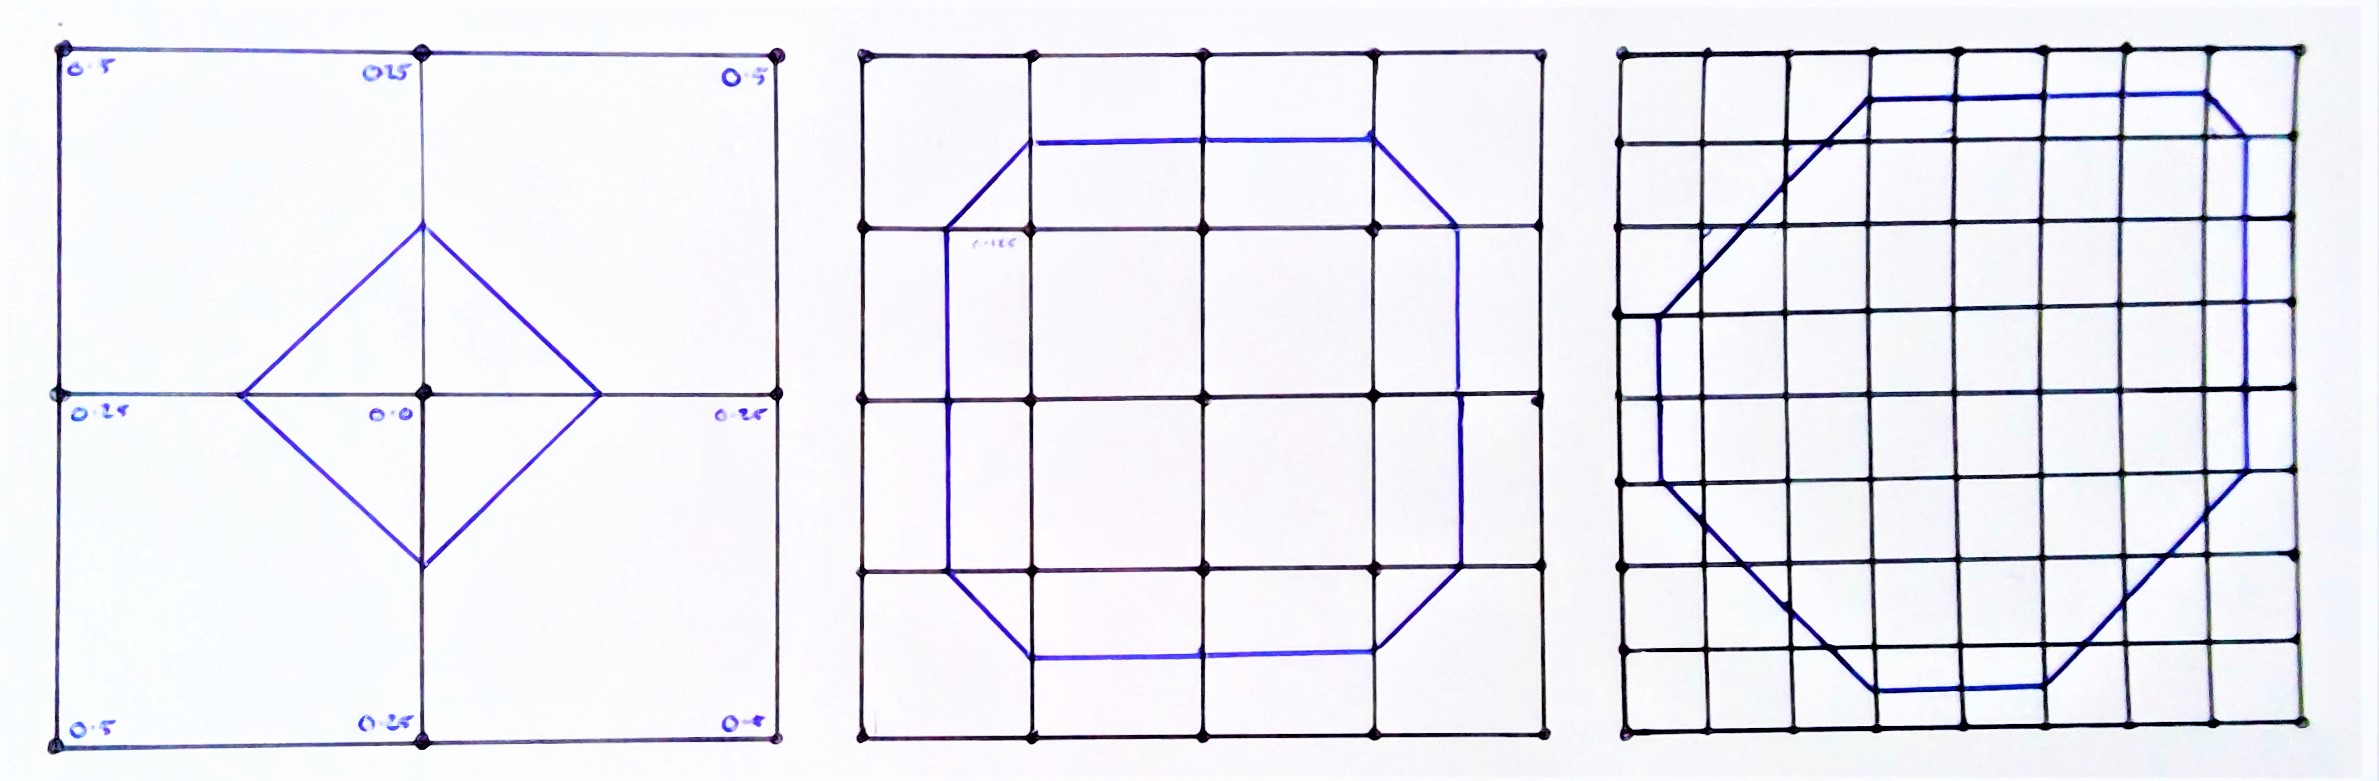
\includegraphics[width=0.9\textwidth]{Marching Squares}
\caption{Bounding curve $f(x,y) = 0.16$, at increasing levels of granularity.}
\label{Marching Squares}
\end{figure}

\vspace{5pt}\noindent
%\newpage\noindent
Consider gridpoints $\mathbf{a}$, $\mathbf{b}$, such that $f_{\mathbf{a}} < c < f_{\mathbf{b}}$. By Figure \ref{Marching Square Partitions}, their partitioning line will bisect edge $AB$ exactly - if the partition is to represent an isoline, then it surely requires $f\left(0.5\mathbf{a} + 0.5\mathbf{b}\right) \approx c$, but this is a rather arbirtrary assumption about the scalar field. Instead making the standard, first-order approximation that $f$ is linear over short distances, it would follow that
$$f\left((1-t)\mathbf{a} + t\mathbf{b}\right) \approx c, \,\, \textrm{where} \,\, t = \frac{c-f_{\mathbf{a}}}{f_{\mathbf{b}}-f_{\mathbf{a}}}.$$
Understanding that it is more accurate for the partition to intersect $AB$ at $(1-t)\mathbf{a} + t\mathbf{b}$, such linear interpolation is integrated into the marching squares algorithm (see Figure \ref{Interpolated Marching Squares}).

\begin{figure}[h]
\centering
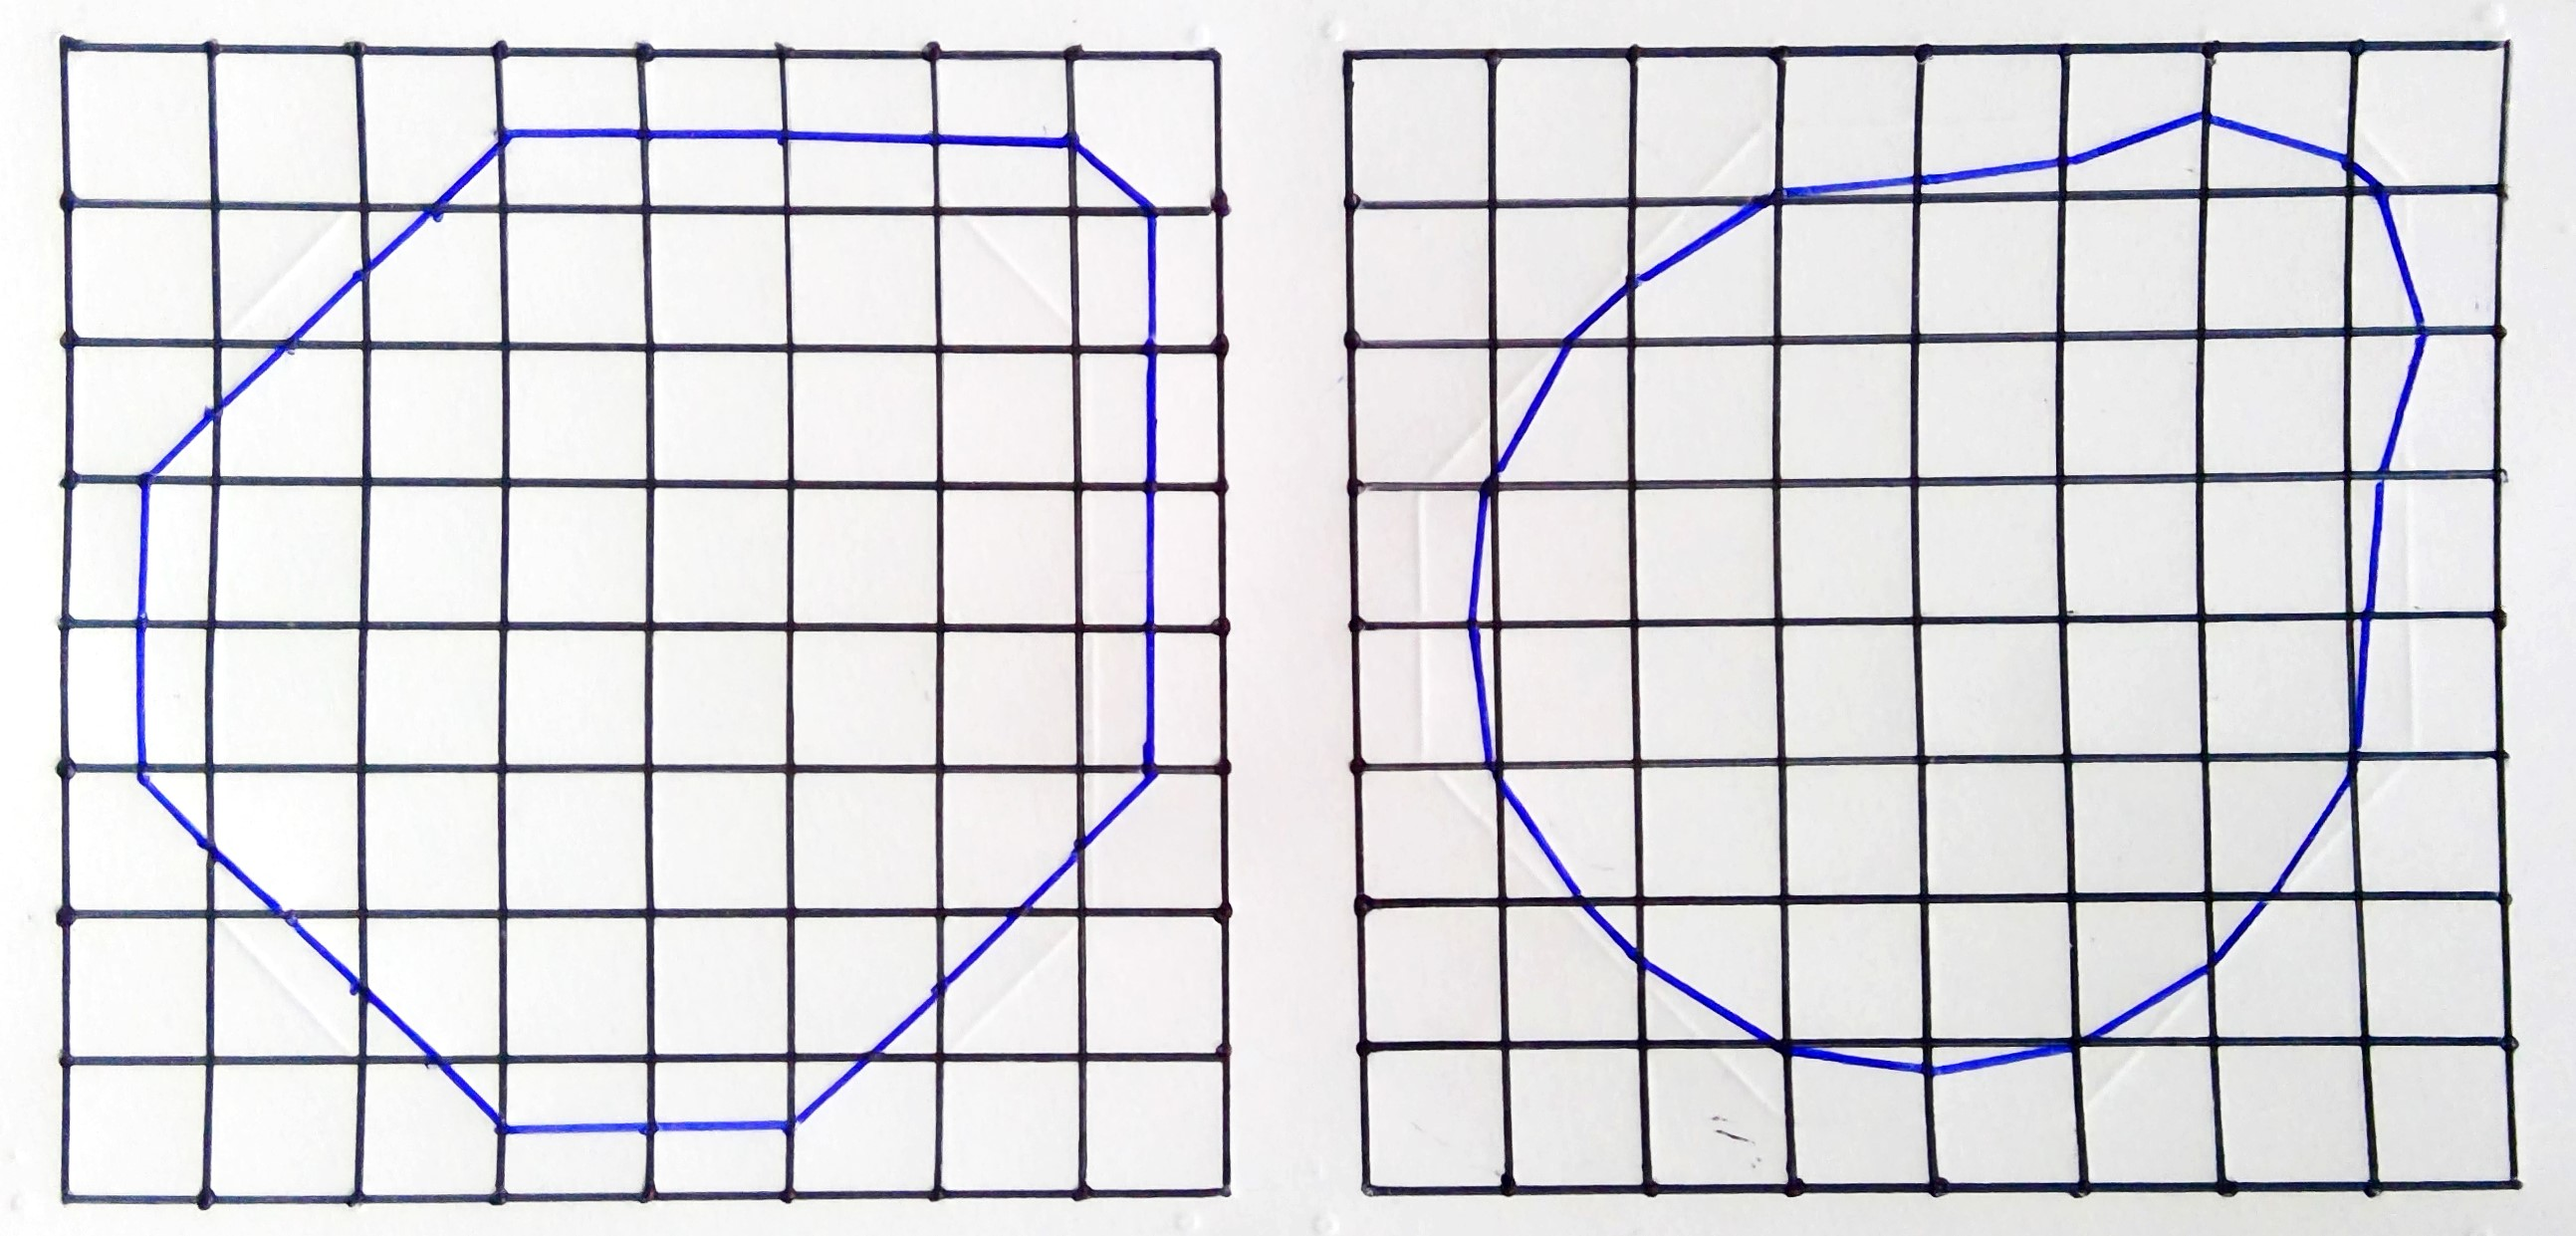
\includegraphics[width=0.9\textwidth]{Interpolated Marching Squares}
\caption{Bounding curve $f(x,y) = 0.16$, before and after linear intepolation.}
\label{Interpolated Marching Squares}
\end{figure}

\vspace{5pt}\noindent
Coming back to the task at hand, then, \textit{Concrete Earth} uses \textit{marching cubes} to generate \textit{isosurfaces} bounding 3D volumes. Partitioning with surfaces... (which, ). [Outside of the expected changes - scalar fields now operate on domain $[0,1]^3$, vertices now have $2^8 = 256$ possible configurations along [the edges of] each marching cube - this is actually a rather straightforward generalisation.]

\vspace{5pt}\noindent
This report will not offer a full breakdown of the 3D algorithm. In particular, the finer points of the DirectX implementation - [breaking down into triangles], or identifying adjacent marching cubes to construct `smooth' vertex normals\footnote{These being averaged from the surface normals of the surrounding faces; if , then it will be weighted by $1/((\mathbf{b}-\mathbf{a})\times(\mathbf{c}-\mathbf{a})) \propto$ the inverse of its area} %, being the weighted average Each [face] [has] [area], [so...].} 
- are deliberately . [Intention of this section, focused on intuition, guiding principle...]. Paul \citeauthor{bourkeMarchingCubes}'s \textit{Polygonising a Scalar Field} \citeyearpar{bourkeMarchingCubes} remains the definitive source on the technique [whereas this report is focused on intuition?]. %... [mention marching tetrahedra? While X, marching cubes have been perfectly adequate for the purposes set out below... save this for the evaluation!].

\subsubsection{Case Study: Hexes}

Having . 3D fields are inherently , yet these are essential to carving out \textit{Concrete Earth}'s landscape.

\vspace{5pt}\noindent
Even a blank hex tile comes with som nuance. [Use of noise...]

\vspace{5pt}\noindent
[Bounding hexagonal prism... As much as flat faces are antithetical to marching cubes (if they run parallel to the grid, then... can't interpolate? notice that interpolation doesn't account for the degenerate case where two adjacent gridpoints are equal)...] 

\subsubsection{Case Study: Landmarks}

\subsection{Procedural Screen Shaders}\label{Procedural Screen Shaders} % TECHNIQUE: L-systems...

The post-processing in \textit{Concrete Earth} is, in many respects, trivial. \texttt{vignette\_ps.hlsl}, for instance, calls only two renders-to-texture on every frame: the board itself, and an alpha map of blood vessels sprouting from the edges of the screen. As striking as the final effect is, the shader is surprisingly straightforward in blending the textures into a single, pulsing eye strain overlay; far more worthy of further discussion is how the blood vessels themselves are generated.

\vspace{5pt}\noindent
In formal languages, a grammar is a tuple $G = (N,\Sigma,P,\omega_0)$. This contains two disjoint sets of symbols: nonterminals $A, B, \dots \in N$, and terminals $a, b, \dots \in \Sigma$. The production rules in $P$ map nonterminals to strings $\alpha, \beta, \dots \in (N\cup\Sigma)^*$; applied recursively to the axiom $\omega_0 \in (N\cup\Sigma)^*$, these rules can produce increasingly complex \textit{sentences} of terminals and/or nonterminals.\footnote{In mathematical literature, $
\omega_0 \in N$ \citep*{hopcroftFormalLanguages}, but \textit{Untitled} takes an informal approach.}

\vspace{5pt}\noindent
The Chomsky hierarchy \citep{chomskyHierarchy} % NB: Is this *strictly* true?
classifies grammars by their production rules:
\begin{enumerate}[label=,itemsep=0em]
\item \textit{Type-3}. \textit{Regular grammars} map $A \mapsto a$ or $A \mapsto aB$.
\item \textit{Type-2}. \textit{Context-free grammars} map $A \mapsto \alpha$.
\item \textit{Type-1}. \textit{Context-sensitive grammars} $\alpha A\beta \mapsto \alpha\gamma\beta$.
\item \textit{Type-0}. \textit{Unrestricted grammars} map $\alpha \mapsto \beta$, where $\alpha$ is non-empty.
\end{enumerate}
Note that all Type-3 grammars are also Type-2, all Type-2 grammars also Type-1, and so on.

\vspace{5pt}\noindent
Suppose, for example, that $N = \{F, G\}$, $\Sigma = \{+, -\}$, $P = \{F \mapsto F+G, G \mapsto F-G\}$, $\omega_0 = F$.
Letting $\omega_n$ denote the sentences generated by applying the production rules $n$ times, it follows that
$$\begin{matrix*}[l]
\omega_1 &= &F+G, \\
\omega_2 &= &F+G+F-G, \\
\omega_3 &= &F+G+F-G+F+G-F-G, \\
\omega_4 &= &F+G+F-G+F+G-F-G+F+G+F-G-F+G-F-G, \;\; \cdots.
\end{matrix*}$$

\vspace{5pt}\noindent
While these defintions are rather abstract, \citet{lindenmayerLSystems} provides a remarkable application. Treating each symbol as an instruction like `go forward' or `turn right', \textit{L-systems} visualise sentences via `turtle graphics'; when those sentences have been generated recursively by a grammar, the line drawings inherit that same self-similar structure. Consider the above, where reading non-terminals $F$, $G$ as `draw a line while moving one unit forwards,' and terminals $\pm$ as `turn $\pm\, \pi/2$ on the spot,' produces the fractal dragon curves in Figure \ref{Dragon Curves}.

%\vspace{5pt}\noindent
\begin{figure}[h]
\centering
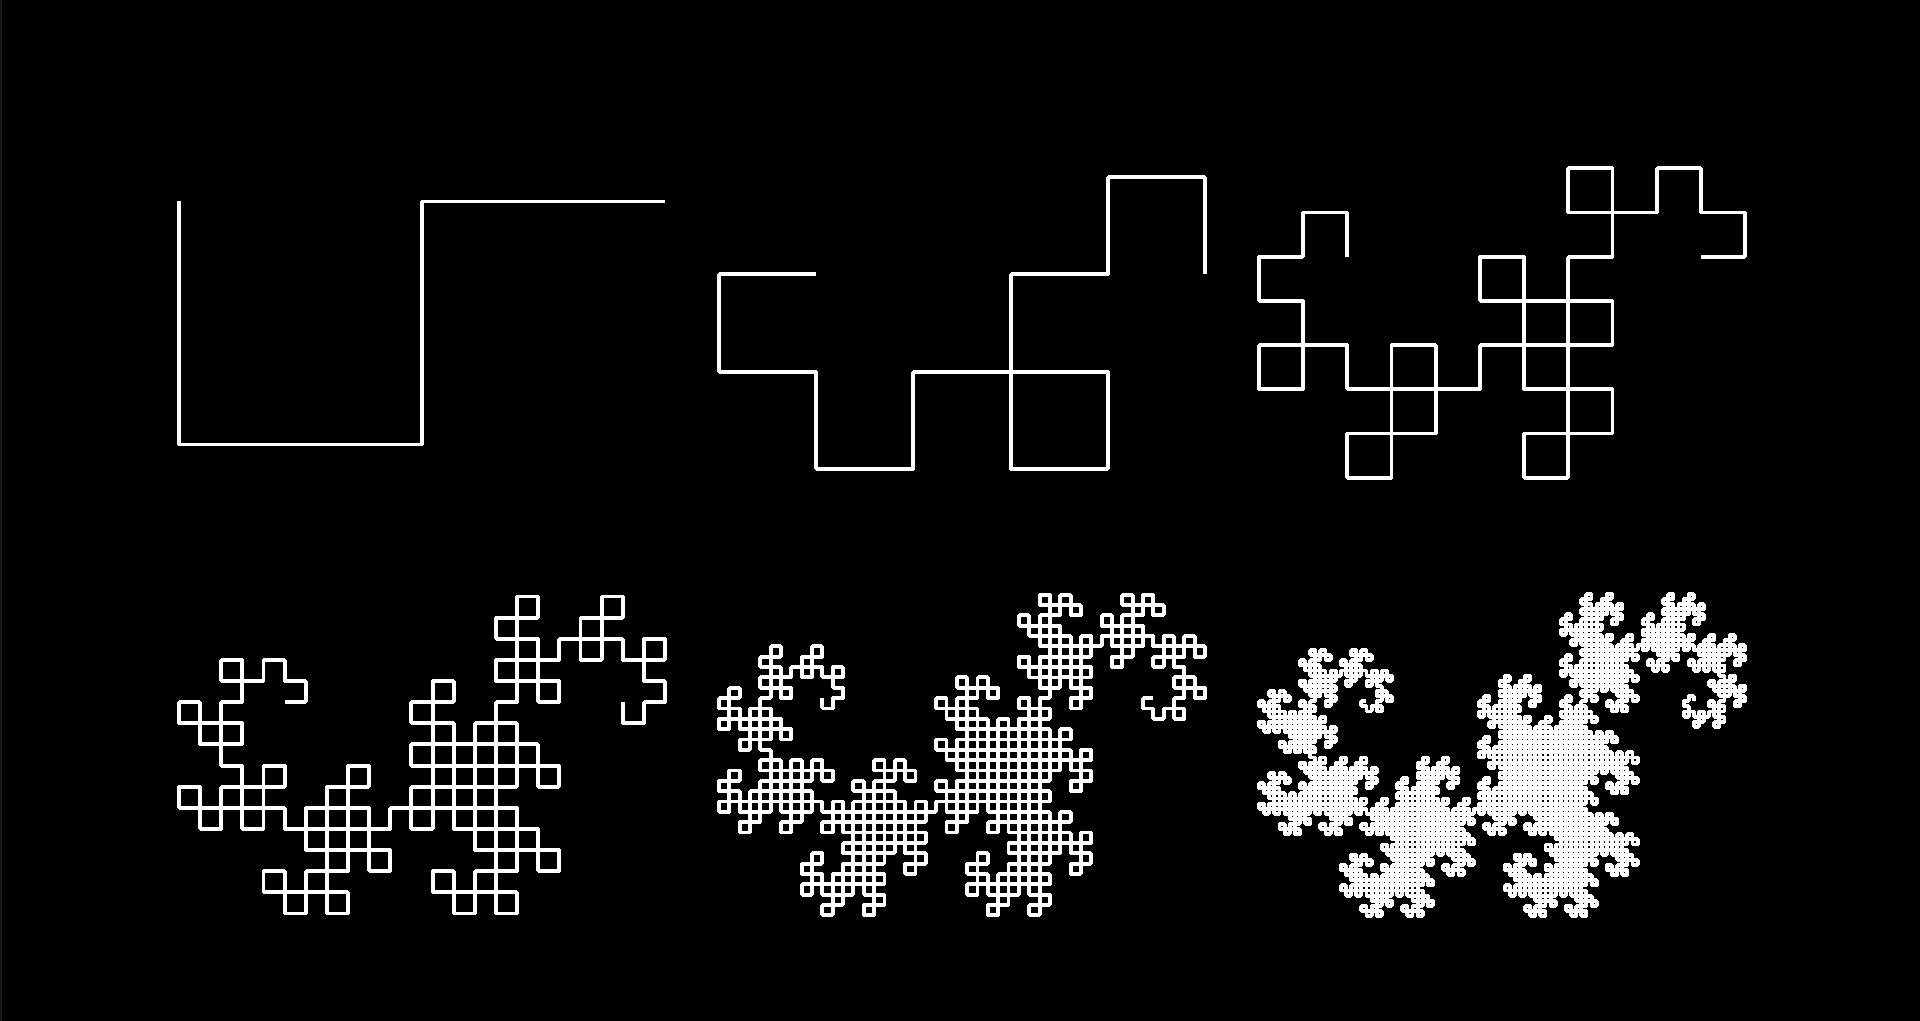
\includegraphics[width=0.66\textwidth]{Dragon Curves}
\caption{Dragon curves, generated by strings $\omega_2, \omega_4, \cdots, \omega_{12}$.}
\label{Dragon Curves}
\end{figure}

\vspace{5pt}\noindent
While L-systems are most common in the modelling of 3D plants and other branching structures \citep{prusinkiewiczAlgorithmicBeauty}, \textit{Untitled} only uses them to generate 2D alpha maps. Moreover, it restricts its attention to L-systems paired with context-free grammars.

\subsubsection{Case Study: Ciphers}

Parametric L-systems \citep{hananParametricLSystems} exist as a generalisation of the above. [theory].

\vspace{5pt}\noindent
The modules in \textit{Concrete Earth}, then, track three . More than anything, this offers a certain clarity of code - at least from a 

\vspace{5pt}\noindent
[Example: various geometric runes!].

\subsubsection{Case Study: Blood Vessels} % Include post-processing!

\citet{zamirArterialBranchingLSystems}, meanwhile, uses parametric L-systems to visualise the bifurcation of blood vessels. Suppose a branch with length $l$, width $w$ bifurcates into two branches $M$ and $m$, such that $l_M \geq l_m$. Defining the \textit{asymmetry ratio} $\alpha = l_m/l_M$, it follows that
$$l_M = \frac{l}{\left(1+\alpha^3\right)^{1/3}}, \;\; l_m = \frac{\alpha\cdot l}{\left(1+\alpha^3\right)^{1/3}}, \;\; w_M = \frac{w}{\left(1+\alpha^3\right)^{1/3}}, \;\; w_m = \frac{\alpha\cdot w}{\left(1+\alpha^3\right)^{1/3}}.$$
Furthermore, the branches diverge from their parent at angles
$$\theta_M = \arccos\left(\frac{\left(1+\alpha^3\right)^{4/3}+1-\alpha^4}{2\left(1+\alpha^3\right)^{2/3}}\right), \;\; \theta_m = \arccos\left(\frac{\left(1+\alpha^3\right)^{4/3}+\alpha^4-1}{2\alpha^2\left(1+\alpha^3\right)^{2/3}}\right).$$
\textit{Untitled}'s framework is therefore capable of reproducing \citeauthor{zamirArterialBranchingLSystems}'s results (see Figure \ref{Zamir Branching}), using an L-system with the single production rule:  
$$\mathbf{C}(l,w,\theta) \mapsto \mathbf{X}(l,w,\theta)[\mathbf{C}(l_M,w_M,\theta+\theta_M)]\mathbf{C}(l_m,w_m,\theta-\theta_m).$$

%\vspace{5pt}\noindent
\begin{figure}[h]
\centering
%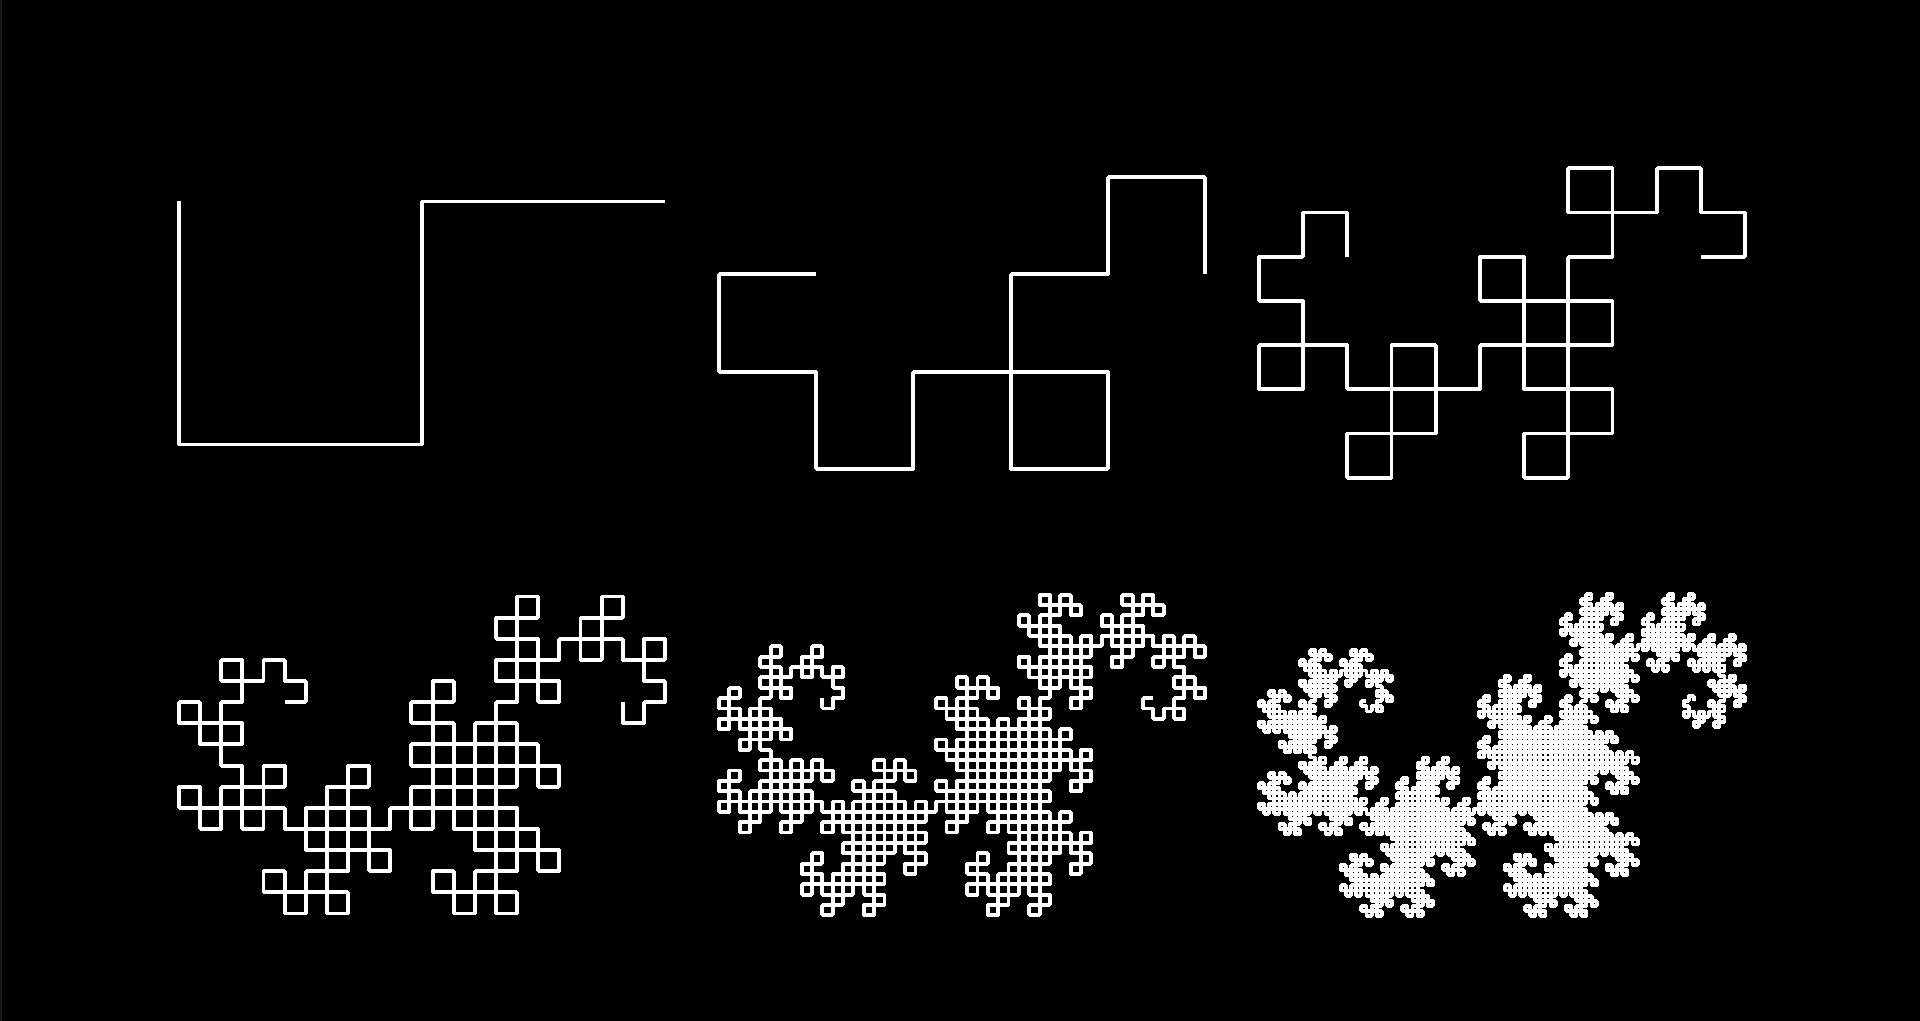
\includegraphics[width=0.66\textwidth]{Dragon Curves}
\caption{\citeauthor{zamirArterialBranchingLSystems}'s model of arterial branching, with asymmetry ratios $\alpha = 1.0, 0.8, \cdots, 0.2$.}
\label{Zamir Branching}
\end{figure}

%\vspace{5pt}\noindent
%$$\begin{matrix*}[l]
%\mathbf{C} &\mapsto &\mathbf{X}[+\mathbf{C}]-\mathbf{C} \\
%\mathbf{X} &\mapsto &\mathbf{X}\mathbf{X}
%\end{matrix*}$$

%\vspace{5pt}\noindent
%$$\begin{matrix*}[l]
%\mathbf{C}, \\
%\mathbf{X}[+\mathbf{C}]-\mathbf{C}, \\
%\mathbf{X}\mathbf{X}[+\mathbf{X}[+\mathbf{C}]-\mathbf{C}]-\mathbf{X}[+\mathbf{C}]-\mathbf{C}, \\
%\mathbf{X}\mathbf{X}\mathbf{X}\mathbf{X}[+\mathbf{X}\mathbf{X}[+\mathbf{X}[+\mathbf{C}]-\mathbf{C}]-\mathbf{X}[+\mathbf{C}]-\mathbf{C}]-\mathbf{X}\mathbf{X}[+\mathbf{X}[+\mathbf{C}]-\mathbf{C}]-\mathbf{X}[+\mathbf{C}]-\mathbf{C}, \;\; \cdots
%\end{matrix*}$$

%\vspace{5pt}\noindent
%$$\begin{matrix*}[l]
%\mathbf{C}(l,w,\theta) &\xmapsto[0.4]{} &\mathbf{X}(l,w,\theta)[\mathbf{C}(l_M,w_M,\theta+\theta_M)]\mathbf{C}(l_m,w_m,\theta-\theta_m) \\
%\mathbf{C}(l,w,\theta) &\xmapsto[0.4]{} &\mathbf{X}(l,w,\theta)[\mathbf{C}(l_m,w_m,\theta+\theta_m)]\mathbf{C}(l_M,w_M,\theta-\theta_M) \\
%\mathbf{C}(l,w,\theta) &\xmapsto[0.2]{} &\mathbf{X}(l,w,\theta)\mathbf{C}(l,w,\theta) \\
%\end{matrix*}$$

\vspace{5pt}\noindent
\citet{liuSimulationBloodVessels} expand on this by introducing a stochastic component - that is to say, they allow [a more random structure]. \textit{Untitled} incorporates such randomness into its own rules for blood vessels:
$$\begin{matrix*}[l]
\mathbf{C}(l,w,\theta) &\xmapsto[0.4]{} &\mathbf{X}(l,w,\theta)[\mathbf{L}(l_M,w_M,\theta+\theta_M)]\mathbf{R}(l_m,w_m,\theta-\theta_m) \\
\mathbf{C}(l,w,\theta) &\xmapsto[0.4]{} &\mathbf{X}(l,w,\theta)[\mathbf{L}(l_m,w_m,\theta+\theta_m)]\mathbf{R}(l_M,w_M,\theta-\theta_M) \\
\mathbf{C}(l,w,\theta) &\xmapsto[0.2]{} &\mathbf{X}(l,w,\theta)\mathbf{C}(l,w,\theta) \\
& & \\
\mathbf{L}(l,w,\theta) &\xmapsto[1.0]{} &\mathbf{X}(l,w,\theta)\mathbf{C}(l_M,w_M,\theta-\theta_M) \\
& & \\
\mathbf{R}(l,w,\theta) &\xmapsto[1.0]{} &\mathbf{X}(l,w,\theta)\mathbf{C}(l_M,w_M,\theta+\theta_M)
\end{matrix*}$$
These describe a capillary with a 40\% chance of bifurcating with branch $M$ tacking clockwise, a 40\% chance of bifurcating with $M$ tacking anticlockwise, and a 20\% chance of extending forwards without any branching. The determinstic production rules on $\mathbf{L}$, $\mathbf{R}$ provide course correction, guaranteeing the [...]; further informal tweaks can be found in the \texttt{LBloodVessel} class, all intended to get the final look of the L-systems `right' (see Figure [reference]). 

\vspace{5pt}\noindent
[Figure of blood vessels in isolation]

\vspace{5pt}\noindent
[Discussion of animation (and the shortcomings thereof)...]

\vspace{5pt}\noindent
[Figure of final render]

\subsection{Procedural Narrative} % TECHNIQUE: 'Improv-lite' text generation...

\textit{Untitled} was originally conceived as a showcase of procedural text generation, an application of [authored X] towards interactive fiction. 

\subsubsection{Grammars}

Given their origin in linguistics, it is perhaps unsurprising that grammars (see Section \ref{Procedural Screen Shaders}) are of use in the field of procedural narrative - \textit{Tracery} \citep{comptonTracery} being the prime example. From a mathematical perspective, this is a stochastic, context-free grammar, with uniformly-distributed production rules for each non-terminal; it iterates a given axiom until all non-terminals (demarcated by \texttt{\{BRACE\}} delimiters) have been replaced. To bemoan the generator as better suited to Twitter bots than immersive storytelling is to misunderstand its design. \citeauthor{comptonTracery} present a lightweight tool that is left \textit{deliberately} narrow, intended for ease-of-use amongst even the most fledgling authors.

\vspace{5pt}\noindent
More substantial works, then, adapt \textit{Tracery}'s grammar-based approach to their own specifications. In \textit{The Annals of the Parrigues}, \citeauthor{shortParrigues} uses a consistent, context-sensitive generator that ``defines any facts about the world that aren’t already defined at the moment of generation'' (\citeyear{shortParrigues}, p. 83). \textit{Voyageur} \citep{diasVoyageur} attaches weightings to the distributions of its production rules \citep{diasVoyageurDescriptions}. Produceral storytelling is an art form; as much as \textit{Concrete Earth} wears these influences on its sleeve, to try and consolidate these into an `optimal', one-size-fits-all generator would be missing the point. This project therefore uses an implementation of \textit{Tracery} with a couple of custom modifications tailored to its own needs.

\paragraph{Recency} [Clear, one sentence goal: avoid unnecessary repetition with recency].\footnote{\textit{Improv}, the generator for \textit{Voyageur}, calls this same quality `dryness'.} \textit{Concrete Earth} defines this by rank: given a non-terminal with $N$ possible production rules, the most recently used rule is will have a recency of $N-1$, the second most recent $N-2$, and so on down to the rule that has been used longest ago (or indeed, never been used), with recency $0$. Though it [does not consider the actual time interval between these uses, nor the \textit{second} most ], this metric is already enough to achieve the desired effect \citep{kazemiSimpleProceduralGeneration}.

\vspace{5pt}\noindent
[Second paragraph: how does this affect weighting?] $p^{n/(N-1)}$, such that (all other weightings being equal), the most recently used rule (with $n = N-1$) will be $p$ times as likely as the least recent ($n = 0$).\footnote{The same string \texttt{alpha} might replace two different non-terminals \texttt{\#A\#}, \texttt{\#B\#}. Recognising these as distinct production rules, the recency with which one was applied to \texttt{\#A\#} has no bearing on when the other is applied to \texttt{\#B\#}, or vice versa.} 

\vspace{5pt}\noindent
Note that [joint recency!].

\paragraph{Characterisation} [Consistency discussion...]

\paragraph{Nested Non-Terminals} [Explain use case...]

\vspace{5pt}\noindent
[Link back to consistency...]

\vspace{5pt}\noindent
This is still too limited, from a dramatic perspective. For all this effort to [maintain consistency], personality is not immutable; so much of good storytelling relies on character \textit{development}.
Indeed, how does the player feel like they have an impact, if [the grammar doesn't have permission to make changes]? \textit{Concrete Earth} surely requires some sort of override...
%Does this make sense, dramaturgically?

\subsubsection{Content Selection Architectures} \textit{Storylets} \citep{kreminskiStorylets} are [definition].

\vspace{5pt}\noindent
In \textit{Concrete Earth}, these storylets are envisioned as the means for these [global changes]. [Discuss a beginning-middle-end structure].%[Though conceptually no different, ... , our `narrative stack'...]
 
\vspace{5pt}\noindent
The current implementation is limited. [Conditions: randomness]. [Effects: entering/exiting the party].

\section{Code Organisation}

Taking a step back, [...].

\vspace{5pt}\noindent
Section \ref{Features} has been structured [to reflect the two fundamental stages of graphics programming: first implementing frameworks (marching cubes, L-systems), then building tangible objects out of them (terrain hexes, blood vessels)]. \textit{Concrete Earth}'s code is structured accordingly. [Using inheritance...]. [Crucially, little is left exposed in the main \textit{Game.cpp} file...].

%Mention use of `tags' in JSON?

\subsection{Rendering}

\subsection{GUI}

[Include HDRR/bloom here...]

\section{Evaluation}\label{Evaluation}

\subsection{Features}

[Start with marching cubes: successful, but more to do...]

\vspace{5pt}\noindent
Marching cubes, too, have been used effectively. T

\vspace{5pt}\noindent
\begin{figure}[h]
\centering

\includegraphics[width=0.66\textwidth]{Euclidean Voronoi Voxel}
\caption{3D Voronoi noise. While voxel textures [would have...]}
\label{Euclidean Voronoi Voxel}
\end{figure}

\vspace{5pt}\noindent
To the extent that \textit{Concrete Earth} has any single `special feature', though, it would surely be its approach to procedural storytelling. [...]

\subsection{Code Organisation}

Built on previous work from CMP502, this project could be written to an already-established style. Functions and variables follow a consistent naming convention, with a strong focus on readability. Inheritance has helped reduce redundancies. Even the current, informal use of comments proves effective, these breaking down the logic behind key snippets, highlighting potential bugs, and overall acting as valuable memos-to-self (a collaborative project would obviously require a higher standard of documentation). In this very granular sense, \textit{Concrete Earth} is a perfectly acceptable piece of code.

\vspace{5pt}\noindent
[Stripping back shaders... an effective strategy!]

\vspace{5pt}\noindent
[Position weakness of the storytelling as an \textit{organisational} matter...]

\vspace{5pt}\noindent
[Discuss the broader merits of Section 4, ultimately landing on the value of \textit{internal consistency}? Or - contrast narrative with models?]

\section{Conclusions}

From a more personal perspective, I can't help but feel that \textit{Concrete Earth} shows promise.

\vspace{5pt}\noindent
[Coheres in a way that my CMP502 project absolutely didn't...]. [Furthermore, a better sense of performance] - I might not be happy with the loading times \textit{per se}, but all things considered these advanced graphics techniques will still run on my laptop.

\vspace{5pt}\noindent
Of course, there is a distinction to be drawn between \textit{Concrete Earth}'s functionality as a graphics showcase and as a game. As much as there's a certain level of interactivity on display,\footnote{And likewise, non-interactive features like the fixed, orthographic camera carry some level of intentionality...} [Perils of interactive narrative].

\vspace{5pt}\noindent
[What/how would I go about cannibalising this? Screen shader first/hexes... narrative much more an early experiment in structuring content selection architectures/context-sensitive grammars...]

\vspace{5pt}\noindent
[$3$rd last: iterating marching cubes, to build intuition... justify own rundown...]

\vspace{5pt}\noindent
[$2$nd last: iterating everything...]

\vspace{5pt}\noindent
[Last: framework does not exist in isolation - tie back to CMP502 to show potential! Shaders being stripped back is a great example...]

\bibliographystyle{agsm}
\bibliography{../../Bibliography/Bibliography}
\addcontentsline{toc}{section}{References}
\end{flushleft}
\end{document}
